\apendice{Especificación de diseño}

\section{Introducción}

En este apartado se describe el diseño de la aplicación desarrollada para la simulación del algoritmo C4.5. El objetivo principal del sistema es mostrar de forma didáctica cómo se construye un árbol de decisión a partir de un conjunto de datos, permitiendo observar tanto el árbol resultante como los cálculos realizados en cada paso.

A diferencia de una implementación básica de ID3, esta aplicación incorpora características propias del algoritmo C4.5, como el uso de \textit{Gain Ratio} como criterio principal de selección, el tratamiento de atributos numéricos mediante umbrales, la gestión de atributos categóricos y booleanos, y una fase posterior de poda del árbol.

El diseño de la aplicación se ha planteado para que el usuario pueda cargar datasets de ejemplo o archivos CSV propios, validar su estructura, construir el árbol paso a paso, analizar las métricas utilizadas en cada nodo y estudiar cómo se simplifica el modelo mediante la poda.

\section{Diseño de datos}

\subsection{Almacenamiento de datasets}

Los datasets de ejemplo se almacenan como archivos CSV \cite{csv_wiki} dentro del directorio de datasets de la aplicación del árbol C4.5. Cada archivo representa un caso de uso distinto, como \textit{leads} inmobiliarios, mantenimiento predictivo, conversión web, concesión de préstamos o rendimiento de estudiantes. En la figura \ref{Fig_C.1} se muestra un ejemplo de como tiene que ser un archivo CSV.

\begin{figure}[htbp]
     \centering
     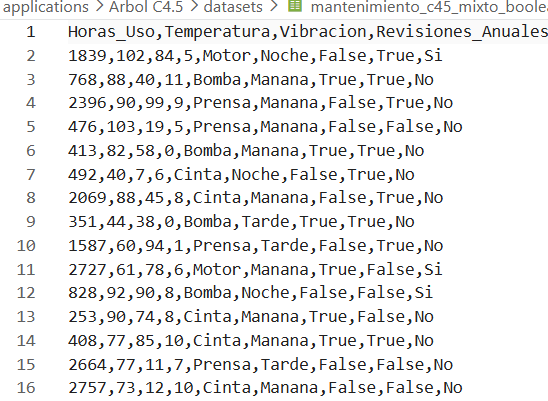
\includegraphics[width=0.75\textwidth]{img/Ejemplo_CSV.png}
     \caption{Visualización de ejemplo de CSV}
     \label{Fig_C.1}
 \end{figure}

La aplicación mantiene una relación entre el nombre visible del dataset y la ruta del archivo correspondiente. Cuando el usuario selecciona un dataset de ejemplo, el sistema lo carga, interpreta su contenido como texto, lo convierte en una matriz de filas y columnas, valida su estructura y genera el modelo C4.5.

El usuario también puede cargar un archivo CSV propio. En este caso, la lectura se realiza localmente en el navegador mediante \texttt{FileReader}, sin necesidad de enviar los datos a un servidor. Esto simplifica la arquitectura y permite que todo el procesamiento se realice en el lado cliente.

\subsection{Formato y restricciones del CSV}

El formato CSV se utiliza porque permite representar datos tabulares de forma sencilla. La primera fila debe contener los nombres de los atributos y las filas siguientes contienen las instancias. La última columna se interpreta siempre como la clase objetivo.

Para asegurar que el simulador pueda procesar los datos correctamente, se aplican las siguientes restricciones:

\begin{itemize}
    \item El archivo debe estar separado por comas.
    \item Debe contener una cabecera y al menos una fila de datos.
    \item La cabecera no puede contener columnas vacías.
    \item Todas las filas deben tener el mismo número de columnas.
    \item No se admiten valores vacíos.
    \item El dataset no puede superar las 150 filas de datos.
    \item El dataset no puede superar las 25 columnas.
    \item La última columna debe ser la clase objetivo.
    \item La clase objetivo debe contener exactamente dos valores distintos.
    \item Los atributos pueden ser numéricos, categóricos o booleanos.
\end{itemize}

Además, la aplicación detecta errores comunes de formato, como archivos separados por punto y coma, tabulaciones o espacios, e informa al usuario de que debe utilizar comas como separador.

La aplicación infiere automáticamente el tipo de cada atributo. Si todos los valores de una columna pueden interpretarse como números, el atributo se considera numérico. Para ello se aceptan valores con punto decimal o coma decimal. Si la columna contiene valores no numéricos, se trata como atributo categórico.

\subsection{Representación del árbol}

Cada nodo del árbol almacena la información necesaria para reconstruir el proceso de decisión. Entre los datos guardados se encuentran el identificador del nodo, el número de registros que llegan a él, la distribución de clases, la entropía, la clase mayoritaria, el atributo seleccionado, el tipo de atributo, el umbral elegido en caso de atributo numérico, la ganancia de información, el \textit{Split Info}, el \textit{Gain Ratio}, los hijos del nodo y la condición de rama que lo conecta con su padre. En las figuras \ref{Fig_C.2} y \ref{Fig_C.3} se muestra una representación de como se visualizan los nodos y hojas en el árbol.

\begin{figure}[htbp]
     \centering
     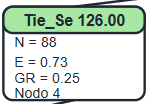
\includegraphics[width=0.25\textwidth]{img/Ejemplo_Nodo.png}
     \caption{Visualización de ejemplo de la representación de un nodo}
     \label{Fig_C.2}
 \end{figure}

 En la figura \ref{Fig_C.2}, se muestra la representación de un nodo con los atributos que se muestran relevantes los cuales son:
 \begin{description}
    \item[N:] Número de datos representados por el nodo.
    \item[E:] Entropía total del nodo.
    \item[GR:] \textit{Gain ratio} del nodo.
    \item[Nodo 4:] Nombre representativo del nodo en el árbol.
\end{description}

 \begin{figure}[htbp]
     \centering
     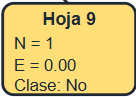
\includegraphics[width=0.25\textwidth]{img/Ejemplo_Hoja.png}
     \caption{Visualización de ejemplo de la representación de una hoja}
     \label{Fig_C.3}
 \end{figure}

  En la figura \ref{Fig_C.3}, se muestra la representación de una hoja con los atributos que se muestran relevantes los cuales son:
 \begin{description}
    \item[N:] Número de datos representados por la hoja.
    \item[E:] Entropía total de la hoja.
    \item[Clase: No] Clase predicha, que se corresponde con la clase mayoritaria del subconjunto asociado.
\end{description}


\section{Diseño arquitectónico}

No se crearon paquetes para este proyecto, ya que las diferentes partes de la aplicación web se almacenaron simplemente en directorios distintos.

No obstante, se procuró extraer en archivos independientes aquellas funciones que se utilizaban en varios archivos JavaScript. De este modo, las funciones específicas podían ser importadas por los archivos que las necesitaban.

\section{Diseño procedimental}

El caso más relevante en relación con el procedimiento y la secuencia de ejecución es aquel en el que un usuario ejecuta el simulador de árboles de decisión C4.5 y ejecuta el simulador de la poda del árbol de decisión C4.5. Las figuras \ref{Fig_C.4} y \ref{Fig_C.5} representan los diagramas de secuencia de las ejecuciones respectivamente.

\begin{figure}[htbp]
     \centering
     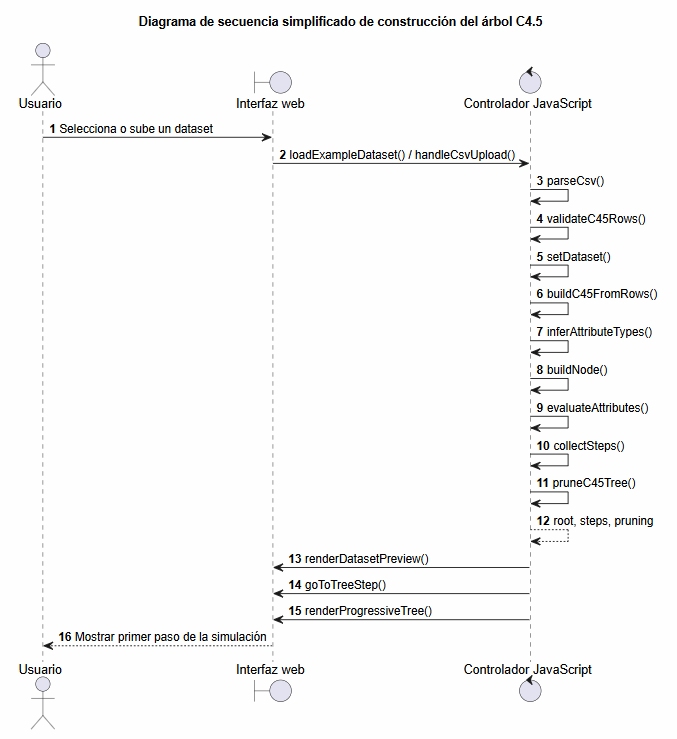
\includegraphics[width=0.75\textwidth]{img/Diagrama_Secuencia_Arbol.png}
     \caption{Visualización del diagrama de secuencia de la generación del árbol}
     \label{Fig_C.4}
 \end{figure}

 \begin{figure}[htbp]
     \centering
     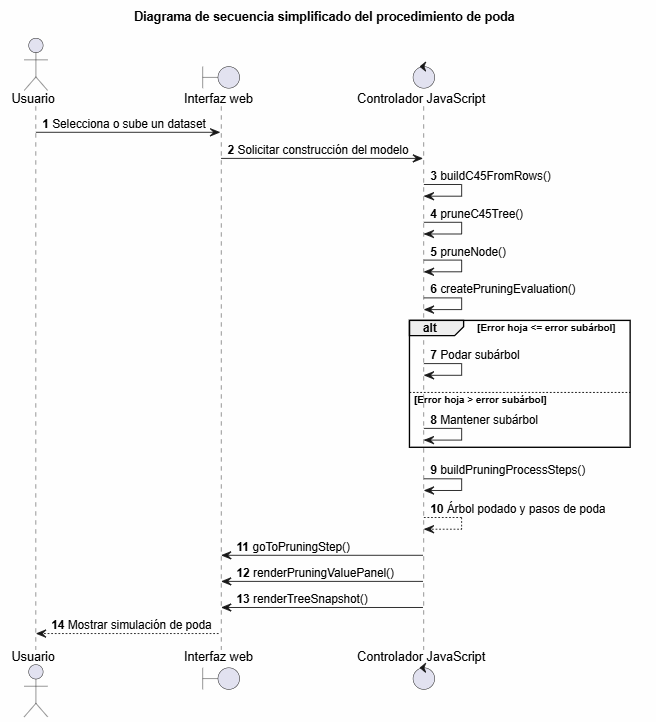
\includegraphics[width=0.75\textwidth]{img/Diagrama_Secuencia_Poda.png}
     \caption{Visualización del diagrama de secuencia de la poda}
     \label{Fig_C.5}
 \end{figure}

En ambos casos, cuando se selecciona un conjunto de datos CSV válido, el programa se asegura de cargar previamente todos los recursos necesarios antes de mostrarlos en pantalla. De este modo, el usuario no tiene que esperar, por ejemplo, a que se cargue la tabla de datos cuando el árbol de decisión en formato SVG ya se ha generado y mostrado.